%%%%%%%%%%%%%%%%%%%%%%%%%%%%%%%%%%%%%%%%%%%%%%%%%%%%%%%%%%%%%%%%
% This intro/reminder comes after a first course on sequence
% processing with 1D NNet for discrete sequence. 
% reminder: sequence of discrete symbols
% - examples of application
% - + exemples of Human activity / audio classification
% - embeddings
% - COnv 1D
% - Pooling

% Alphabet = set of nucleotides: 
% A,C,G,T
\newcommand{\cga}{{\color{red!70!black} A}}
\newcommand{\cgc}{{\color{blue!70!black} C}}
\newcommand{\cgg}{{\color{yellow!70!black} G}}
\newcommand{\cgt}{{\color{green!70!black} T}}

\begin{frame}{Sequence of discrete symbols classification }
  \begin{block}{Movie review classification}
    \begin{center}
      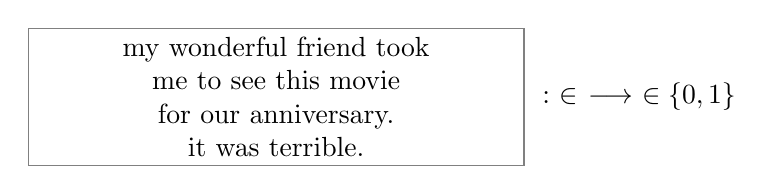
\begin{tikzpicture}
        %%%%%%%%%%%%%%%%%%%%% 
        \node[anchor=east,draw=gray,text width=0.5\textwidth,align=center] (review) at
        (0,0) {my wonderful friend took me to see this movie \\for our
          anniversary. \\ it was terrible.};
        %%%%%%%%%%%%%%%%%%%%% 
        \node[anchor=west] (txt) at (0.1,0) {$: \ \x \in \real^{\nfeats} \ \longrightarrow \ \class \in\{0, 1\}$};
      \end{tikzpicture}
    \end{center}
  \end{block}
  \begin{block}{Enhancer Identification in  DNA Sequences}
    \begin{center}
      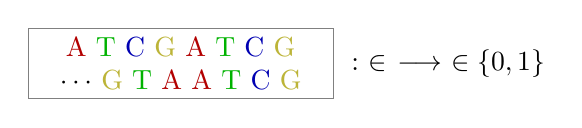
\begin{tikzpicture}
        %%%%%%%%%%%%%%%%%%%%% 
        \node[anchor=east,draw=gray,text width=0.3\textwidth,align=center] (review) at
        (0,0) {\cga~\cgt~\cgc~\cgg~\cga~\cgt~\cgc~\cgg\\$\cdots$~\cgg~\cgt~\cga~\cga~\cgt~\cgc~\cgg};
        %%%%%%%%%%%%%%%%%%%%% 
        \node[anchor=west] (txt) at (0.1,0) {$: \ \x \in \real^{\nfeats} \ \longrightarrow \ \class \in\{0, 1\}$};
      \end{tikzpicture}
    \end{center}
  \end{block}
  \begin{itemize}
  \item $\dataset= (\exi , \classi )_{i=1}^{\nsamples}$ 
  \item The input is a sequence $\rightarrow$ how to build $\x$ ? 
  \item A sequence of discrete symbols $\in \vocab$
  \item Symbols  interact with each other, the neighborhood is important
  \end{itemize}
\end{frame}


%%%%%%%%%%%%%%%%%%%%%%%%%%%%%%%%%%%%%%%%%%%%%%%%%%%%%%%%%%%%%%%%%%
\begin{frame}{Embedding of discrete symbols}
    \begin{center}
      \begin{displaymath}
          \begin{array}{lcccccccc}
            \seq{s}=&[ &\cgc&\cga&\cgt&\cgt&\cgg&\cgt
                        &]\\
            &&\downarrow &\downarrow &\downarrow &\downarrow &\downarrow &\downarrow \\
            \textrm{Look-up}&&\wemb &\wemb &\wemb &\wemb &\wemb &\wemb  \\
               &&\wvector_{\cgc}&\wvector_{\cga}&\wvector_{\cgt}&\wvector_{\cgt}&\wvector_{\cgg}&\wvector_{\cgt} \\
          \end{array}
        \end{displaymath}
        {\huge $\downarrow$} \\
        \tikz{\draw[step=0.5,black,thin] (0,0) grid (3,2);}
    \end{center}
\end{frame}

%%%%%%%%%%%%%%%%%%%%%%%%%%%%%%%%%%%%%%%%%%%%%%%%%%%%%%%%%%%%%%%%%%
% In pytorch the indices are :
% batch, channel, data-point
% The data point for a 1D input is (t,d)
% For an image it is (x,y)
\begin{frame}{Convolution 1D}
  \framesubtitle{Extract a frame, or a window, and apply a ``filter''}
  \begin{columns}
    \column{0.6\textwidth}
    %%% the input : a matrix + window
    \begin{center}
    The input sequence of  $L=6$ \\vectors in $\real^{\nfeats}$,  $\nfeats=4$ \\[1ex]
    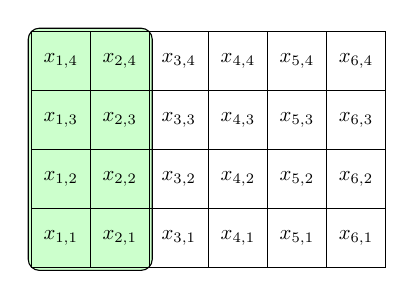
\begin{tikzpicture}[scale=0.75,every node/.style={scale=0.75}]
      % the window
      % offset for x and y of .5 + a bit more 
      \draw[fill=green!20,rounded corners] (0.45,0.45) rectangle (2.55,4.55); % green 
      %% the grid 
      \foreach \l in {1,2,...,4}
      \foreach \c in {1,2,...,6}
      {
        \draw (\c,\l) +(-.5,-.5) rectangle ++(.5,.5);
        \draw (\c,\l) node{$x_{\c,\l}$};
      }
    \end{tikzpicture}
  \end{center}
    \column{0.6\textwidth}
    \begin{center}
    The filter:\\kernel size of $ks=2$\\[1ex]
    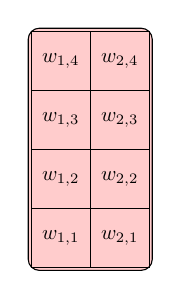
\begin{tikzpicture}[scale=0.75,every node/.style={scale=0.75}]
      % the window
      % offset for x and y of .5 + a bit more 
      \draw[fill=red!20,rounded corners] (0.45,0.45) rectangle (2.55,4.55); % green 
      
      %% the grid 
      \foreach \l in {1,2,...,4}
      \foreach \c in {1,2}
      {
        \draw (\c,\l) +(-.5,-.5) rectangle ++(.5,.5);
        \draw (\c,\l) node{$w_{\c,\l}$};
      }
    \end{tikzpicture}
  \end{center}
\end{columns}
\begin{block}{The output value (output channel)}
  $$
  \textrm{At time }t = 1,\ {\color{red!70!black} h_1} = \sum_{i,j} {\color{red!70!black}w_{i,j}}\times  {\color{green!70!black}x_{i,j}}
  $$
\end{block}
\end{frame}



%%%%%%%%%%%%%%%%%%%%%%%%%%%%%%%%%%%%%%%%%%%%%%%%%%%%%%%%%%%%%%%%%%%%%%%%%%%%%%%%%%%%%%%% 
\begin{frame}{Convolution 1D}
  \framesubtitle{With 2 output channels}
  \begin{columns}
    \column{0.6\textwidth}
    %%% the input : a matrix + window
    \begin{center}
      $L=6$,  $\nfeats=4$ \\[1ex]
      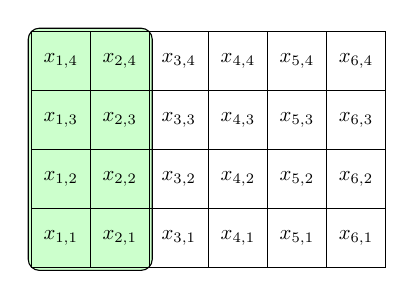
\begin{tikzpicture}[scale=0.75,every node/.style={scale=0.75}]
        % the window
        % offset for x and y of .5 + a bit more 
        \draw[fill=green!20,rounded corners] (0.45,0.45) rectangle (2.55,4.55); % green 
        %% the grid 
        \foreach \l in {1,2,...,4}
        \foreach \c in {1,2,...,6}
        {
          \draw (\c,\l) +(-.5,-.5) rectangle ++(.5,.5);
          \draw (\c,\l) node{$x_{\c,\l}$};
        }
      \end{tikzpicture}
    \end{center}
    \column{0.4\textwidth}
    \begin{center}
      Filters:kernel size of $ks=2$\\[1ex]
      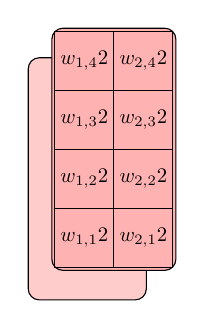
\begin{tikzpicture}[scale=0.75,every node/.style={scale=0.75}]
        % the window
        % offset for x and y of .5 + a bit more 
        \draw[fill=red!20,rounded corners] (0.05,-0.05) rectangle (2.05,4.05); % first 
        \draw[fill=red!30,rounded corners] (0.45,0.45) rectangle (2.55,4.55); 
        %% the grid 
        \foreach \l in {1,2,...,4}
        \foreach \c in {1,2}
        {
          \draw (\c,\l) +(-.5,-.5) rectangle ++(.5,.5);
          \draw (\c,\l) node{$w_{\c,\l}\lid{2}$};
        }
      \end{tikzpicture}
    \end{center}
  \end{columns}
  \begin{block}{The output value (output channel)}
    \begin{align*}
      {\color{red!70!black} h_{1,1}} &= \sum_{i,j} {\color{red!70!black}w_{i,j}\lid{1}}\times  {\color{green!70!black}x_{i,j}} \\
      {\color{red!70!black} h_{2,1}} &= \sum_{i,j} {\color{red!70!black}w_{i,j}\lid{2}}\times  {\color{green!70!black}x_{i,j}} 
    \end{align*}
  \end{block}
\end{frame}



